\section{Theory} \label{sec:theory}

\subsection{Linear regression}
In linear regression, the dependent variable $y_i$ is a linear combination of the parameters, and for a dependent variable this can be written as
	\begin{equation}
	y_i=\sum_jX_{ij}\beta_j.
	\end{equation}
	In principle, $x_{ij}$ can be an arbitrary function of the arguments $x_i$, and in this project the $x_{ij}$'s are all spin interactions in the Ising model ($x_{ij}=s_is_j$).
	
	We will study Ordinary Least Square (OLS) regression, Ridge regression and Lasso regression. The OLS cost function is known as
	\begin{equation}
	c(\vec{\beta})=\sum_{i=1}^{n}\Big(y_i-\beta_0-\sum_{j=1}^px_{ij}\beta_j\Big)^2\qquad\qquad\qquad\text{OLS}
	\end{equation}
	which is minimized when
	\begin{equation}
	\vec{\beta}=(\hat{X}^T\hat{X})^{-1}\hat{X}^T\vec{y}.
	\end{equation}
	Similarly, the Ridge cost function is
	\begin{equation}
	c(\vec{\beta})=\sum_{i=1}^{n}\Big(y_i-\beta_0-\sum_{j=1}^px_{ij}\beta_j\Big)^2+\lambda\sum_{j=1}^p\beta_j^2\qquad\text{Ridge}
	\end{equation}
	which is minimized when
	\begin{equation}
	\vec{\beta}=(\hat{X}^T\hat{X}+\lambda I)^{-1}\hat{X}^T\vec{y},
	\end{equation}
	and finally the Lasso cost function is given by
	\begin{equation}
	c(\vec{\beta})=\sum_{i=1}^{n}\Big(y_i-\beta_0-\sum_{j=1}^px_{ij}\beta_j\Big)^2+\lambda\sum_{j=1}^p\beta_j\qquad\text{Lasso}.
	\end{equation}
Linear regression is detailed in the project 1 report, [1].


\subsection{Logistic regression}
Despite its name, logistic regression is not a fitting tool, but rather a classification tool. Traditionally, it has been denoted as a single perceptron, and is in some ways a very simple neural network. A perceptron is like a flexible function, where a set of inputs are sent into the network, and a set of outputs is returned. The inputs are multiplied by several weights, and by adjusting those weights a single perceptron can solve every \textit{linear problem} (we come back to this later). A drawing of the perceptron is found in figure (\ref{fig:single_perceptron}).

\begin{figure} [H]
	\centering
	\begin{tikzpicture}
	\node[functions] (center) {};
	\node[below of=center,font=\scriptsize,text width=4em] {Activation function};
	\draw[thick] (0.5em,0.5em) -- (0,0.5em) -- (0,-0.5em) -- (-0.5em,-0.5em);
	\draw (0em,0.75em) -- (0em,-0.75em);
	\draw (0.75em,0em) -- (-0.75em,0em);
	\node[right of=center] (right) {};
	\path[draw,->] (center) -- (right);
	\node[functions,left=3em of center] (left) {$\sum$};
	\path[draw,->] (left) -- (center);
	\node[weights,left=3em of left] (2) {$w_2$} -- (2) node[input,left of=2] (l2) {$x_2$};
	\path[draw,->] (l2) -- (2);
	\path[draw,->] (2) -- (left);
	\node[below of=2] (dots) {$\vdots$} -- (dots) node[left of=dots] (ldots) {$\vdots$};
	\node[weights,below of=dots] (n) {$w_n$} -- (n) node[input,left of=n] (ln) {$x_n$};
	\path[draw,->] (ln) -- (n);
	\path[draw,->] (n) -- (left);
	\node[weights,above of=2] (1) {$w_1$} -- (1) node[input,left of=1] (l1) {$x_1$};
	\path[draw,->] (l1) -- (1);
	\path[draw,->] (1) -- (left);
	\node[weights,above of=1] (0) {$b$} -- (0) node[input,left of=0] (l0) {$B$};
	\node[right of=0,font=\scriptsize] {BIAS};
	\path[draw,->] (l0) -- (0);
	\path[draw,->] (0) -- (left);
	\node[below of=ln,font=\scriptsize] {inputs};
	\node[below of=n,font=\scriptsize] {weights};
	\end{tikzpicture}
	\caption{Logistic regression model with $n$ inputs.}
	\label{fig:single_perceptron}
\end{figure}

Initially, one needs to train the network such that it knows which outputs are correct, and for that one needs to know the outputs that correspond to the inputs. Every time the network is trained, the weights are adjusted such that the error is minimized.

The very first step is to calculate the initial outputs, where the weights usually are set to small random numbers. Then the error is calculated, and the weights are updated to minimize the error. So far so good.

\subsubsection{Forward phase}\label{sec:forward}
Let us look at it from a mathematical perspective, and calculate the net output. The net output seen from an output node is simply the sum of all the "arrows" that point towards the node, see figure (\ref{fig:single_perceptron}), where each "arrow" is given by the left-hand node multiplied with its respective weight. For example, the contribution from input node 2 to the output node follows from $X_2\cdot w_{2}$, and the total net output to the output $O$ is therefore
\begin{empheq}[box={\mybluebox[5pt]}]{equation}
	net = \sum_{i=1}^{I} x_i\cdot w_i + b\cdot 1.
	\label{eq:forward}
\end{empheq}
Just some notation remarks: $x_i$ is the value of input node $i$ and $w_{i}$ is the weight which connects input $i$ to the output. $b$ is the bias weight, which we will discuss later.

You might wonder why we talk about the net output all the time, do we have other outputs? If we look at the network mathematically, what we talk about as the net output should be our only output. Anyway, to make the algorithm easy to implement, mapping the net output to a final output is standard practice. You do not need to care too much about this right now, the mapping is done with an activation function and is explained further in section \ref{sec:sigmoid1}. The activation function, $f$, takes in the net output and gives the output, 
\begin{equation}
out = f(net).
\end{equation}
If not everything is clear right now, it is fine. We will discuss the most important concepts before we dive into the maths.

\subsubsection{BIAS}
As mentioned above, we use biases when calculating the outputs. The nodes, with value $B$, are called the bias nodes, and the weights, $b$, are called the bias weights. But why do we need those? 

Suppose we have two inputs of value zero, and one output which should not be zero (this could for instance be a NOR gate). Without the bias, we will not be able to get any other output than zero, and in fact the network would struggle to find the right weights even if the output had been zero. 

The bias value $B$ does not really matter since the network will adjust the bias weights with respect to it, and is usually set to 1 and ignored in the calculations. [2]

\subsubsection{Learning rate}
In principle, the weights could be updated without adding any learning rate ($\eta=1$), but this can in practice be problematic. It is easy to imagine that the outputs can be fluctuating around the targets without decreasing the error, which is not ideal, and a learning rate can be added to avoid this. The downside is that with a low learning rate the network needs more training to obtain the correct results (and it takes more time), so we need to find a balance. 

\subsubsection{Cost function}\label{sec:cost_function}
The cost function is what defines the error, and we could in principle have used OLS, ridge and so on. However, in logistic regression, the cross-entropy function is known to give good results and we will mainly stick to it:
\begin{empheq}[box={\mybluebox[5pt]}]{equation}
c(\boldsymbol{W}) = -\sum_{i=1}^n\Big[y_i\log f(\boldsymbol{x}_i^T\boldsymbol{W})+(1-y_i)\log[1-f(\boldsymbol{x}_i^T\boldsymbol{W})]\Big]
\label{eq:cross_entropy}
\end{empheq}
where $\boldsymbol{W}$ contains all weights, included the bias weight ($\bb{W}\equiv[b,\bb{W}]$), and similarly does $\bb{x}$ include the bias node, which is 1; $\bb{x}\equiv[1,\bb{x}]$. Further, the $f(x)$ is the logistic function 
\begin{equation}
f(x)=\frac{1}{1+e^{-x}}.
\label{eq:logistic}
\end{equation}

\subsubsection{Activation function}\label{sec:sigmoid1}
Above, we were talking about the activation function, which is used to activate the net output. In binary models, this is often just a step function firing when the net output is above a threshold. For continuous outputs, the logistic function written in equation \eqref{eq:logistic} has traditionally been used as the activation function inspired by neuroscience. This function maps an arbitrary number between 0 and 1, which ensures that the outputs will not explode, and its that derivative has an easy form. The derivative of this function is
\begin{equation}
f'(x)=f(1-f)
\end{equation}
and the derivation of it is shown carefully in Appendix A. The function is presented in figure (\ref{fig:activation_functions}), along with more modern activation functions such as \textit{standard RELU, leaky RELU and ELU}.

\begin{figure}
	\centering
	\subfloat[Sigmoid]{{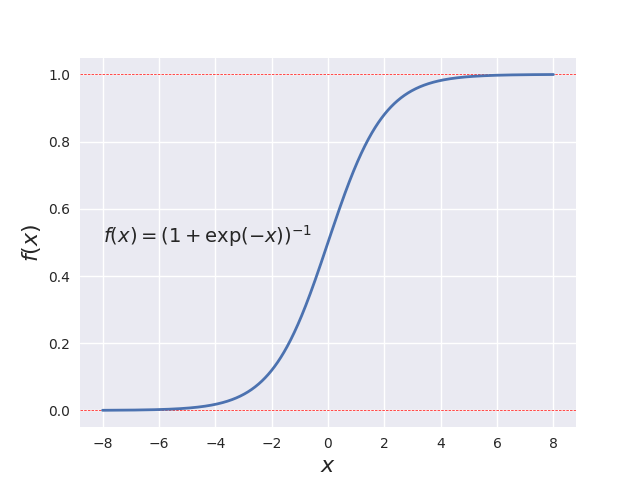
\includegraphics[width=8cm]{../plots/sigmoid.png} }}
	\subfloat[ReLU]{{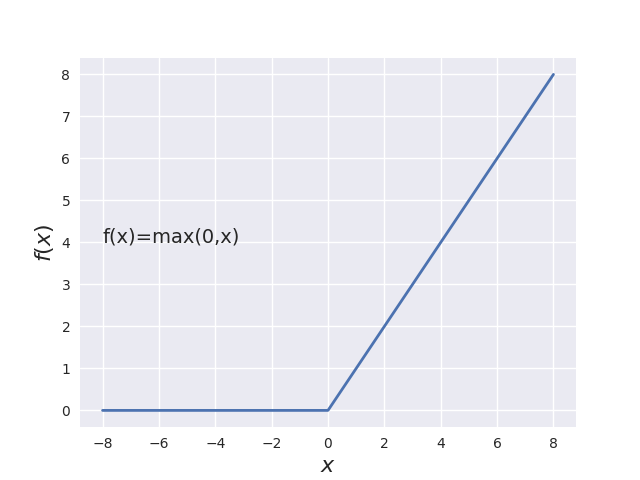
\includegraphics[width=8cm]{../plots/ReLU.png} }}\\
	
	\subfloat[Leaky ReLU]{{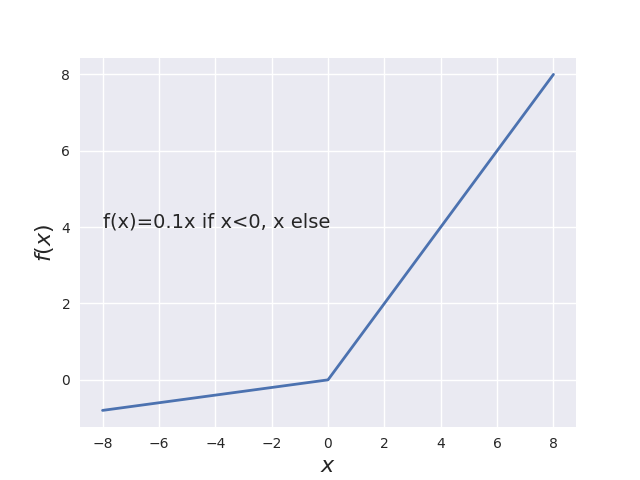
\includegraphics[width=8cm]{../plots/LeakyReLU.png} }}%
	\subfloat[ELU]{{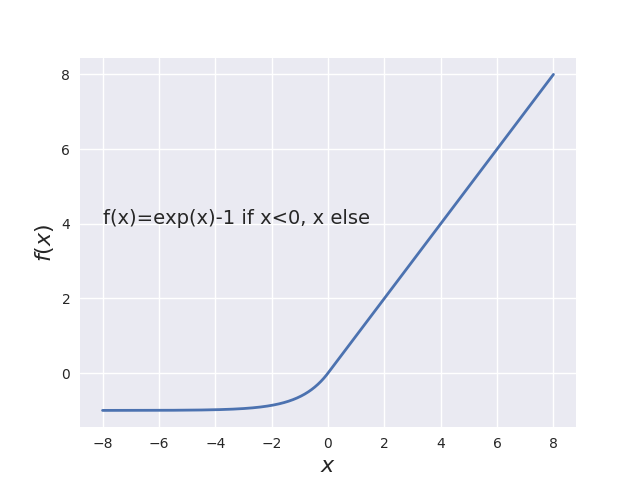
\includegraphics[width=8cm]{../plots/ELU.png} }}
	\caption{Some more or less popular activation functions}%
	\label{fig:activation_functions}%
\end{figure}

\subsubsection{Backward phase}
Now all the tools for finding the outputs are in place, and we can calculate the error. If the outputs are larger than the targets (which are the exact results), the weights need to be reduced, and if the error is large the weights need to be adjusted a lot. The weight adjustment can be done by any minimization method, and we will look at a few gradient methods. To illustrate the point, we will stick to the \textbf{gradient descent} (GD) method in the calculations, even though other methods will be used later. The principle of GD is easy: each weight is "moved" in the direction of steepest slope,
\begin{empheq}[box={\mybluebox[5pt]}]{equation}
\bb{w}^+= \bb{w} - \eta\cdot\frac{\partial c(\boldsymbol{w})}{\partial \bb{w}},
\label{eq:w_update}
\end{empheq}
where $\eta$ is the learning rate and $c(\bb{w})$ is the cost function. 

To go further, we need to choose a cost function which we can differentiate with respect to the weights $\bb{w}$. We choose the one we discussed in section \ref{sec:cost_function}, which has a derivative 
\begin{equation}
\frac{\partial c(\bb{w})}{\partial \bb{w}}=[f(\bb{x}^T\bb{w})-\bb{y}]\bb{x}
\end{equation}
(see Appendix A). The weight update algorithm we use is thus
\begin{empheq}[box={\mybluebox[5pt]}]{align}
\bb{w}^+= \bb{w} - \eta\cdot[f(\bb{x}^T\bb{w})-\bb{y}]\bb{x}.
\end{empheq}
where the bias weight is included implicitly in $\bb{w}$ and the same applies for $\bb{x}$.

\subsubsection{Constraints}
It is naturally that such a simple algorithm has constraints, and in fact it is only able to solve so-called linear problems. The logic functions, such as OR, NOR, AND and NAND are common examples, which all can be implemented using logistic regression. On the other hand, logistic regression is not capable of recognize non-linear functions, such as the XOR-gate. For that we need a neural network, or traditionally called a multi-layer perceptron. 


\subsection{Neural network}
If you have understood logistic regression, understanding a neural network should not be a difficult task. According to  \textbf{the universal approximation theorem}, a neural network with only one hidden layer can approximate any continuous function. [REFERENCE] However, often multiple layers are used since this often causes a fewer total number of nodes. 

In figure \eqref{fig:neural_network}, a two-layer neural network (one hidden layer) is illustrated. It has some similarities with the single perceptron model in figure \eqref{fig:single_perceptron}, but the hidden layer and multiple outputs is added. 

\begin{figure} [H]
	\centering
	\begin{tikzpicture}
	
	% Define outputs
	\node[] (center) {};
	\node[input, above=0.3em of center] (o1) {$o_1$};
	\node[input, below=0.3em of center] (o2) {$o_2$};
	
	% Draw lines from output nodes
	\node[right of=o1] (righto1) {};
	\node[right of=o2] (righto2) {};
	\path[draw,->] (o1) -- (righto1);
	\path[draw,->] (o2) -- (righto2);
	
	% Hidden nodes
	\node[input,left=5em of center] (h3) {$h_3$};
	\node[input,above of=h3] (h2) {$h_2$};
	\node[input,above of=h2] (h1) {$h_1$};
	\node[input,below of=h3] (h4) {$h_4$};
	\node[input,below of=h4] (h5) {$h_5$};
	\node[input,above of=h1] (b2) {$b_2$};
	
	% Draw lines from hidden nodes
	\path[draw,->] (h1) -- (o1);
	\path[draw,->] (h2) -- (o1);
	\path[draw,->] (h3) -- (o1);
	\path[draw,->] (h4) -- (o1);
	\path[draw,->] (h5) -- (o1);
	\path[draw,->] (b2) -- (o1);
	
	\path[draw,->] (h1) -- (o2);
	\path[draw,->] (h2) -- (o2);
	\path[draw,->] (h3) -- (o2);
	\path[draw,->] (h4) -- (o2);
	\path[draw,->] (h5) -- (o2);
	\path[draw,->] (b2) -- (o2);
	
	% Define place left of left
	\node[input,left=5em of h3] (x2) {$x_2$};
	\node[input,above of=x2] (x1) {$x_1$};
	\node[input,below of=x2] (x3) {$x_3$};
	\node[input,above of=x1] (b1) {$b_1$};
	
	% Draw lines from input nodes
	\path[draw,->] (x1) -- (h1);
	\path[draw,->] (x1) -- (h2);
	\path[draw,->] (x1) -- (h3);
	\path[draw,->] (x1) -- (h4);
	\path[draw,->] (x1) -- (h5);
	
	\path[draw,->] (x2) -- (h1);
	\path[draw,->] (x2) -- (h2);
	\path[draw,->] (x2) -- (h3);
	\path[draw,->] (x2) -- (h4);
	\path[draw,->] (x2) -- (h5);
	
	\path[draw,->] (x3) -- (h1);
	\path[draw,->] (x3) -- (h2);
	\path[draw,->] (x3) -- (h3);
	\path[draw,->] (x3) -- (h4);
	\path[draw,->] (x3) -- (h5);
	
	\path[draw,->] (b1) -- (h1);
	\path[draw,->] (b1) -- (h2);
	\path[draw,->] (b1) -- (h3);
	\path[draw,->] (b1) -- (h4);
	\path[draw,->] (b1) -- (h5);
	
	% Draw lines towards input nodes
	\node[left of=x1] (leftx1) {};
	\node[left of=x2] (leftx2) {};
	\node[left of=x3] (leftx3) {};
	\path[draw,->] (leftx1) -- (x1);
	\path[draw,->] (leftx2) -- (x2);
	\path[draw,->] (leftx3) -- (x3);
	
	% Add some text
	\node[below=5.1em of x2,font=\scriptsize] {input};
	\node[below=5em of h3,font=\scriptsize] {hidden};
	\node[below=5.8em of center,font=\scriptsize] {output};
	\end{tikzpicture}
	\caption{Neural network with 3 input nodes, 5 hidden nodes and 2 output nodes, in addition to the bias nodes.}
	\label{fig:neural_network}
\end{figure}

For the single perceptron, the update of weights was quite straight forward, but for a perceptron consisting of multiple layers the question is: how do we update the weights when we do not know the value of the hidden nodes? And how do we know which layer causing the error? This will be explained in section \ref{sec:backward}, where one of the most popular techniques for that is discussed. Before that we will generalize the forward phase presented in logistic regression.

\subsubsection{Forward phase}
In section \ref{sec:forward}, we saw how the output is found for a single perceptron. Since we only had one output node, the weights could be stored in an array. When it comes to a neural network, it is more convenient to store the weights in matrices, since they will have indices related to both the node on left-hand side and the node on the right-hand side. For instance, the weight between input node $x_3$ and hidden node $h_5$ in figure \eqref{fig:neural_network} is usually labeled as $w_{35}$. Since we have two layers, we also need to denote which weight set it belongs to, which we will do by a superscript ($w_{35}\Rightarrow w_{35}^{(1)}$). In the same way, $\bb{W}^1$ is the matrix containing all $w_{ij}^{(1)}$, $\bb{x}$ is the vector containing all $x_i$'s and so on. We then find the net outputs at the hidden layer to be
\begin{empheq}{equation}
net_{h,j} = \sum_{i=1}^{I} x_i\cdot w_{ij}^{(1)}=\bb{x}^T\bb{W}^{(1)}
\label{eq:forward_hidden}
\end{empheq}
where the $\bb{x}$ and $\bb{W}^{(1)}$ again are understood to take the biases. This will be the case henceforth. The real output to the hidden nodes will be
\begin{equation}
h_j = f(net_{h,j}).
\end{equation}
Further, we need to find the net output to the output nodes, which is obviously just
\begin{empheq}{equation}
net_{o,j} = \sum_{i=1}^{H} h_i\cdot w_{ij}^{(2)}=\bb{h}^T\bb{W}^{(2)}
\label{eq:forward_output}
\end{empheq}
We can easily generalize this. Looking at the net output to a hidden layer $l$, we get
\begin{empheq}[box={\mybluebox[5pt]}]{equation}
net_{h_l,j} = \bb{h^{(l-1)}}^T\bb{W}^{(l)}.
\label{eq:forward_general}
\end{empheq}

\subsubsection{Backward Propagation} \label{sec:backward}
Backward propagation is probably the most used technique to update the weights, and is actually again based on equation (\ref{eq:w_update}). What differs, is the differentiation of the cost function, which gets more complex as we add more layers. For one and two hidden layers, we calculate 

We recognize the first part as $\delta_{ok}$, such that
\begin{empheq}[box={\mybluebox[5pt]}]{equation}
w_{ij}^{(1)}\rightarrow w_{ij}^{(1)} - \eta\cdot\sum_{k=1}^{O}\delta_{ok}\cdot w_{jk}^{(2)}\cdot out_{hj}(1-out_{hj})\cdot x_i
\end{empheq}
where we recall $\delta_{ok}$ as
\begin{equation*}
\delta_{ok}=-(t_{ok}-out_{ok})\cdot out_{ok}(1-out_{ok}).
\end{equation*}

\subsubsection{Summary}
Since it will be quite a lot calculations, I will just express the results here, and move the calculations to Appendix C. Let us start with the forward propagation:
\begin{empheq}[box={\mybluebox[5pt]}]{align}
net_{hi}&=\sum_jw_{ji}^{(1)}\cdot i_j + b_{1i}\cdot 1\notag\\
out_{hi}&=\text{sig}(net_{hi})\notag\\
\notag\\
net_{ki}&=\sum_jw_{ji}^{(2)}\cdot out_{hj} + b_{2i}\cdot 1\\
out_{ki}&=\text{sig}(net_{ki})\notag\\
\notag\\
net_{oi}&=\sum_jw_{ji}^{(3)}\cdot out_{kj} + b_{3i}\cdot 1\notag\\
out_{oi}&=\text{sig}(net_{oi})\notag
\end{empheq}
which can easily be turned into vector form. The backward propagation follows from the two-layer example, and we get
\begin{empheq}[box={\mybluebox[5pt]}]{align}
w_{ij}^{(3)}&=w_{ij}^{(3)}-\eta\cdot\delta_{oj}\cdot out_{ki}\notag\\
\notag\\
w_{ij}^{(2)}&=w_{ij}^{(2)}-\eta\sum_{k=1}^O\delta_{ok}\cdot w_{jk}^{(3)}\cdot out_{kj}(1-out_{kj})\cdot out_{hi}\notag\\
\notag\\
w_{ij}^{(1)}&=w_{ij}^{(1)}-\eta\sum_{k=1}^O\sum_{l=1}^K\delta_{ok}\cdot w_{lk}^{(3)}\cdot out_{kl}(1-out_{kl})\cdot w_{jl}^{(2)}out_{hj}(1-out_{hj})\cdot x_i\notag
\end{empheq}
where we again use the short hand 
\begin{equation*}
\delta_{oj}=(t_j-out_{oj})\cdot out_{oj}(1-out_{oj}).
\end{equation*}
If we compare with the weight update formulas for the two-layer case, we recognize some obvious connections, and it is easy to imagine how we can construct a general weight update algorithm, no matter how many layers we have. 

Now over to the problem we want to solve using neural networks.

\subsection{Ising model}
The Ising model is widely used to study phenomena in statistics, physics, economics etc.. In one dimension, it can be viewed as a sequence of two binary numbers, for instance $\pm1$, which we will call spins. Each element interacts with its nearest neighbors by the formula
\begin{equation}
E_{i,i+1}=J_{i,i+1}s_is_{i+1}
\end{equation}
where $s_i$ and $s_{i+1}$ are the values of the respective elements and $J_{i,i+1}$ is the interaction coefficient. The total energy of an Ising model is just the sum of all interaction energies, which becomes
\begin{equation}
E=\sum_iJ_{i,i+1}s_is_{i+1}.
\end{equation}
This particular model is basically setting the interaction between two non-neighbors to zero, but we could generalize this:
\begin{equation}
E=\sum_{ij}J_{i,j}s_is_j.
\end{equation}
where $J$ now is an interaction matrix. We recognize this as an inner product where $\bb{x}$ is a vector containing all $s_is_j$ elements and $\bb{J}$ as the $J$-matrix discussed above flatten out,
\begin{equation}
E=\bb{x}^T\bb{J}.
\end{equation}
We could extend this to a system of $n$ Ising models, by introducing a matrix $\bb{X}=[\bb{x}_1, \bb{x}_2,\hdots,\bb{x}_n]$ which contains all $\bb{x}$-vectors
\begin{equation}
\bb{E}=\bb{X}^T\bb{J}.
\end{equation}
If we now know the spin configuration of the models ($\bb{X}$) and the corresponding energies, we can estimate the $\bb{J}$-vector using linear regression.